
\hypertarget{menu_format}{}
\section{Format}
\index{format menu}

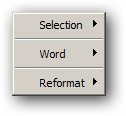
\includegraphics[scale=0.50]{./res/menu_format.png}\\

\begin{scriptsize}\begin{tabularx}{\textwidth}{>{\hsize=0.3\hsize}X>{\hsize=0.7\hsize}X}\\
    \hline
    \textbf{Option} & \textbf{Description} \\
    \hline
    Selection & \textit{\htmladdnormallink{See options ...}{\#menu\_format\_selection}} \\
    Word & \textit{\htmladdnormallink{See options ...}{\#menu\_format\_word}} \\
    Reformat & \textit{\htmladdnormallink{See options ...}{\#menu\_format\_reformat}} \\
    \hline
  \end{tabularx}\end{scriptsize}


\hypertarget{menu_format_selection}{}
\subsection{Selection}
\index{format menu!selection}

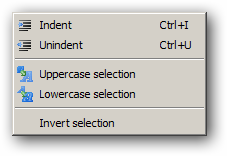
\includegraphics[scale=0.50]{./res/menu_format_selection.png}\\

\begin{scriptsize}\begin{tabularx}{\textwidth}{>{\hsize=0.4\hsize}X>{\hsize=0.6\hsize}X}\\
    \hline
    \textbf{Option} & \textbf{Description} \\
    \hline
    Indent & Indents selected line(s) \\
    Unindent & Unindents selected line(s) \\
    Uppercase selection & Converts selected text into upper case \\
    Lowercase selection & Converts selected text into lower case \\
    Invert selection & Inverts the case of all selected text \\
    \hline
  \end{tabularx}\end{scriptsize}


\hypertarget{menu_format_word}{}
\subsection{Word}
\index{format menu!word}

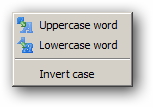
\includegraphics[scale=0.50]{./res/menu_format_word.png}\\

\begin{scriptsize}\begin{tabularx}{\textwidth}{>{\hsize=0.3\hsize}X>{\hsize=0.7\hsize}X}\\
    \hline
    \textbf{Option} & \textbf{Description} \\
    \hline
    Uppercase word & Converts the word under the cursor to upper case \\
    Lowercase word & Converts the word under the cursor to lower case \\
    Invert case & Inverts the case of the word under the cursor \\
    \hline
  \end{tabularx}\end{scriptsize}

\hypertarget{menu_format_reformat}{}
\subsection{Reformat}

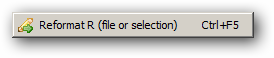
\includegraphics[scale=0.50]{./res/menu_format_reformat.png}


\begin{scriptsize}\begin{tabularx}{\textwidth}{>{\hsize=0.3\hsize}X>{\hsize=0.7\hsize}X}\\
    \hline
    \textbf{Option} & \textbf{Description} \\
    \hline
    Reformat R (file or selection) & Reformat a whole file or selection by using formatR package \\
    \hline
  \end{tabularx}\end{scriptsize}
